\documentclass[titlepage,a4paper]{article}

\usepackage{a4wide}
\usepackage[colorlinks=true,linkcolor=black,urlcolor=blue,bookmarksopen=true]{hyperref}
\usepackage{amsmath}
\usepackage{bookmark}
\usepackage{fancyhdr}
\usepackage[spanish]{babel}
\usepackage[utf8]{inputenc}
\usepackage[T1]{fontenc}
\usepackage{graphicx}
\usepackage{float}
\pagestyle{fancy} % Encabezado y pie de página
\fancyhf{}
\fancyhead[L]{TP2 - Grupo 4}
\fancyhead[R]{Algoritmos y Programación III - FIUBA}
\renewcommand{\headrulewidth}{0.4pt}
\fancyfoot[C]{\thepage}
\renewcommand{\footrulewidth}{0.4pt}

\begin{document}
\begin{titlepage} % Carátula
	\hfill
\includegraphics[width=6cm]{img/logofiuba.jpg}
    \centering
    \vfill
    \Huge \textbf{Trabajo Práctico 2 - Algohoot\\ Entrega 3}
    \vskip2cm
    \Large [7507/9502] Algoritmos y Programación III\\
    Curso 1\\ % Curso 1 para el de la tarde y 2 para el de la noche
    Primer cuatrimestre de 2020 
    \vfill
    \textbf{Grupo 4:}\\$ $\\
    \begin{tabular}{  l  } % Datos del alumno
      Kovnat, Leoni, Locatelli, Rosenblatt y Venglar. %Orden alfabético
  	\end{tabular}
    \vfill
    \vfill
\end{titlepage}

\tableofcontents % Índice general
\newpage

\section{Introducción}\label{sec:intro}
El presente informe reune la documentación de la solución del segundo trabajo práctico de la materia Algoritmos y Programación III que consiste en implementar el juego de trivia Kahoot, denominado por nosotros como Algohoot, utilizando los conceptos del paradigma de la orientación a objetos vistos hasta ahora en el curso.

\section{Supuestos}\label{sec:supuestos}
% Deberá contener explicaciones de cada uno de los supuestos que el alumno haya tenido que adoptar a partir de situaciones que no estén contempladas en la especificación.

\subsection{Puntaje Negativo}

Un jugador admite puntaje negativo si responde mal una pregunta con penalidad y tiene puntaje nulo. 

\subsection{Carga de Datos}

Suponemos mejor no cargar los datos de los jugadores desde un botón en el menú, sino, previo a 
las rondas de preguntas. Además, si se ingresa algún jugador y se vuelve al menú inicial, se eliminarán todos los jugadores ingresados.

\section{Diagramas de Clases}\label{sec:diagramasdeclase}
% Uno o varios diagramas de clases mostrando las relaciones estáticas entre las clases.  Puede agregarse todo el texto necesario para aclarar y explicar su diseño. Recuerden que la idea de todo el documento es que quede documentado y entendible cómo está implementada la solución.

Dejamos a continuación el diagrama de clases que representa las relaciones establecidas hasta el momento:

\begin{figure}[H]
\centering
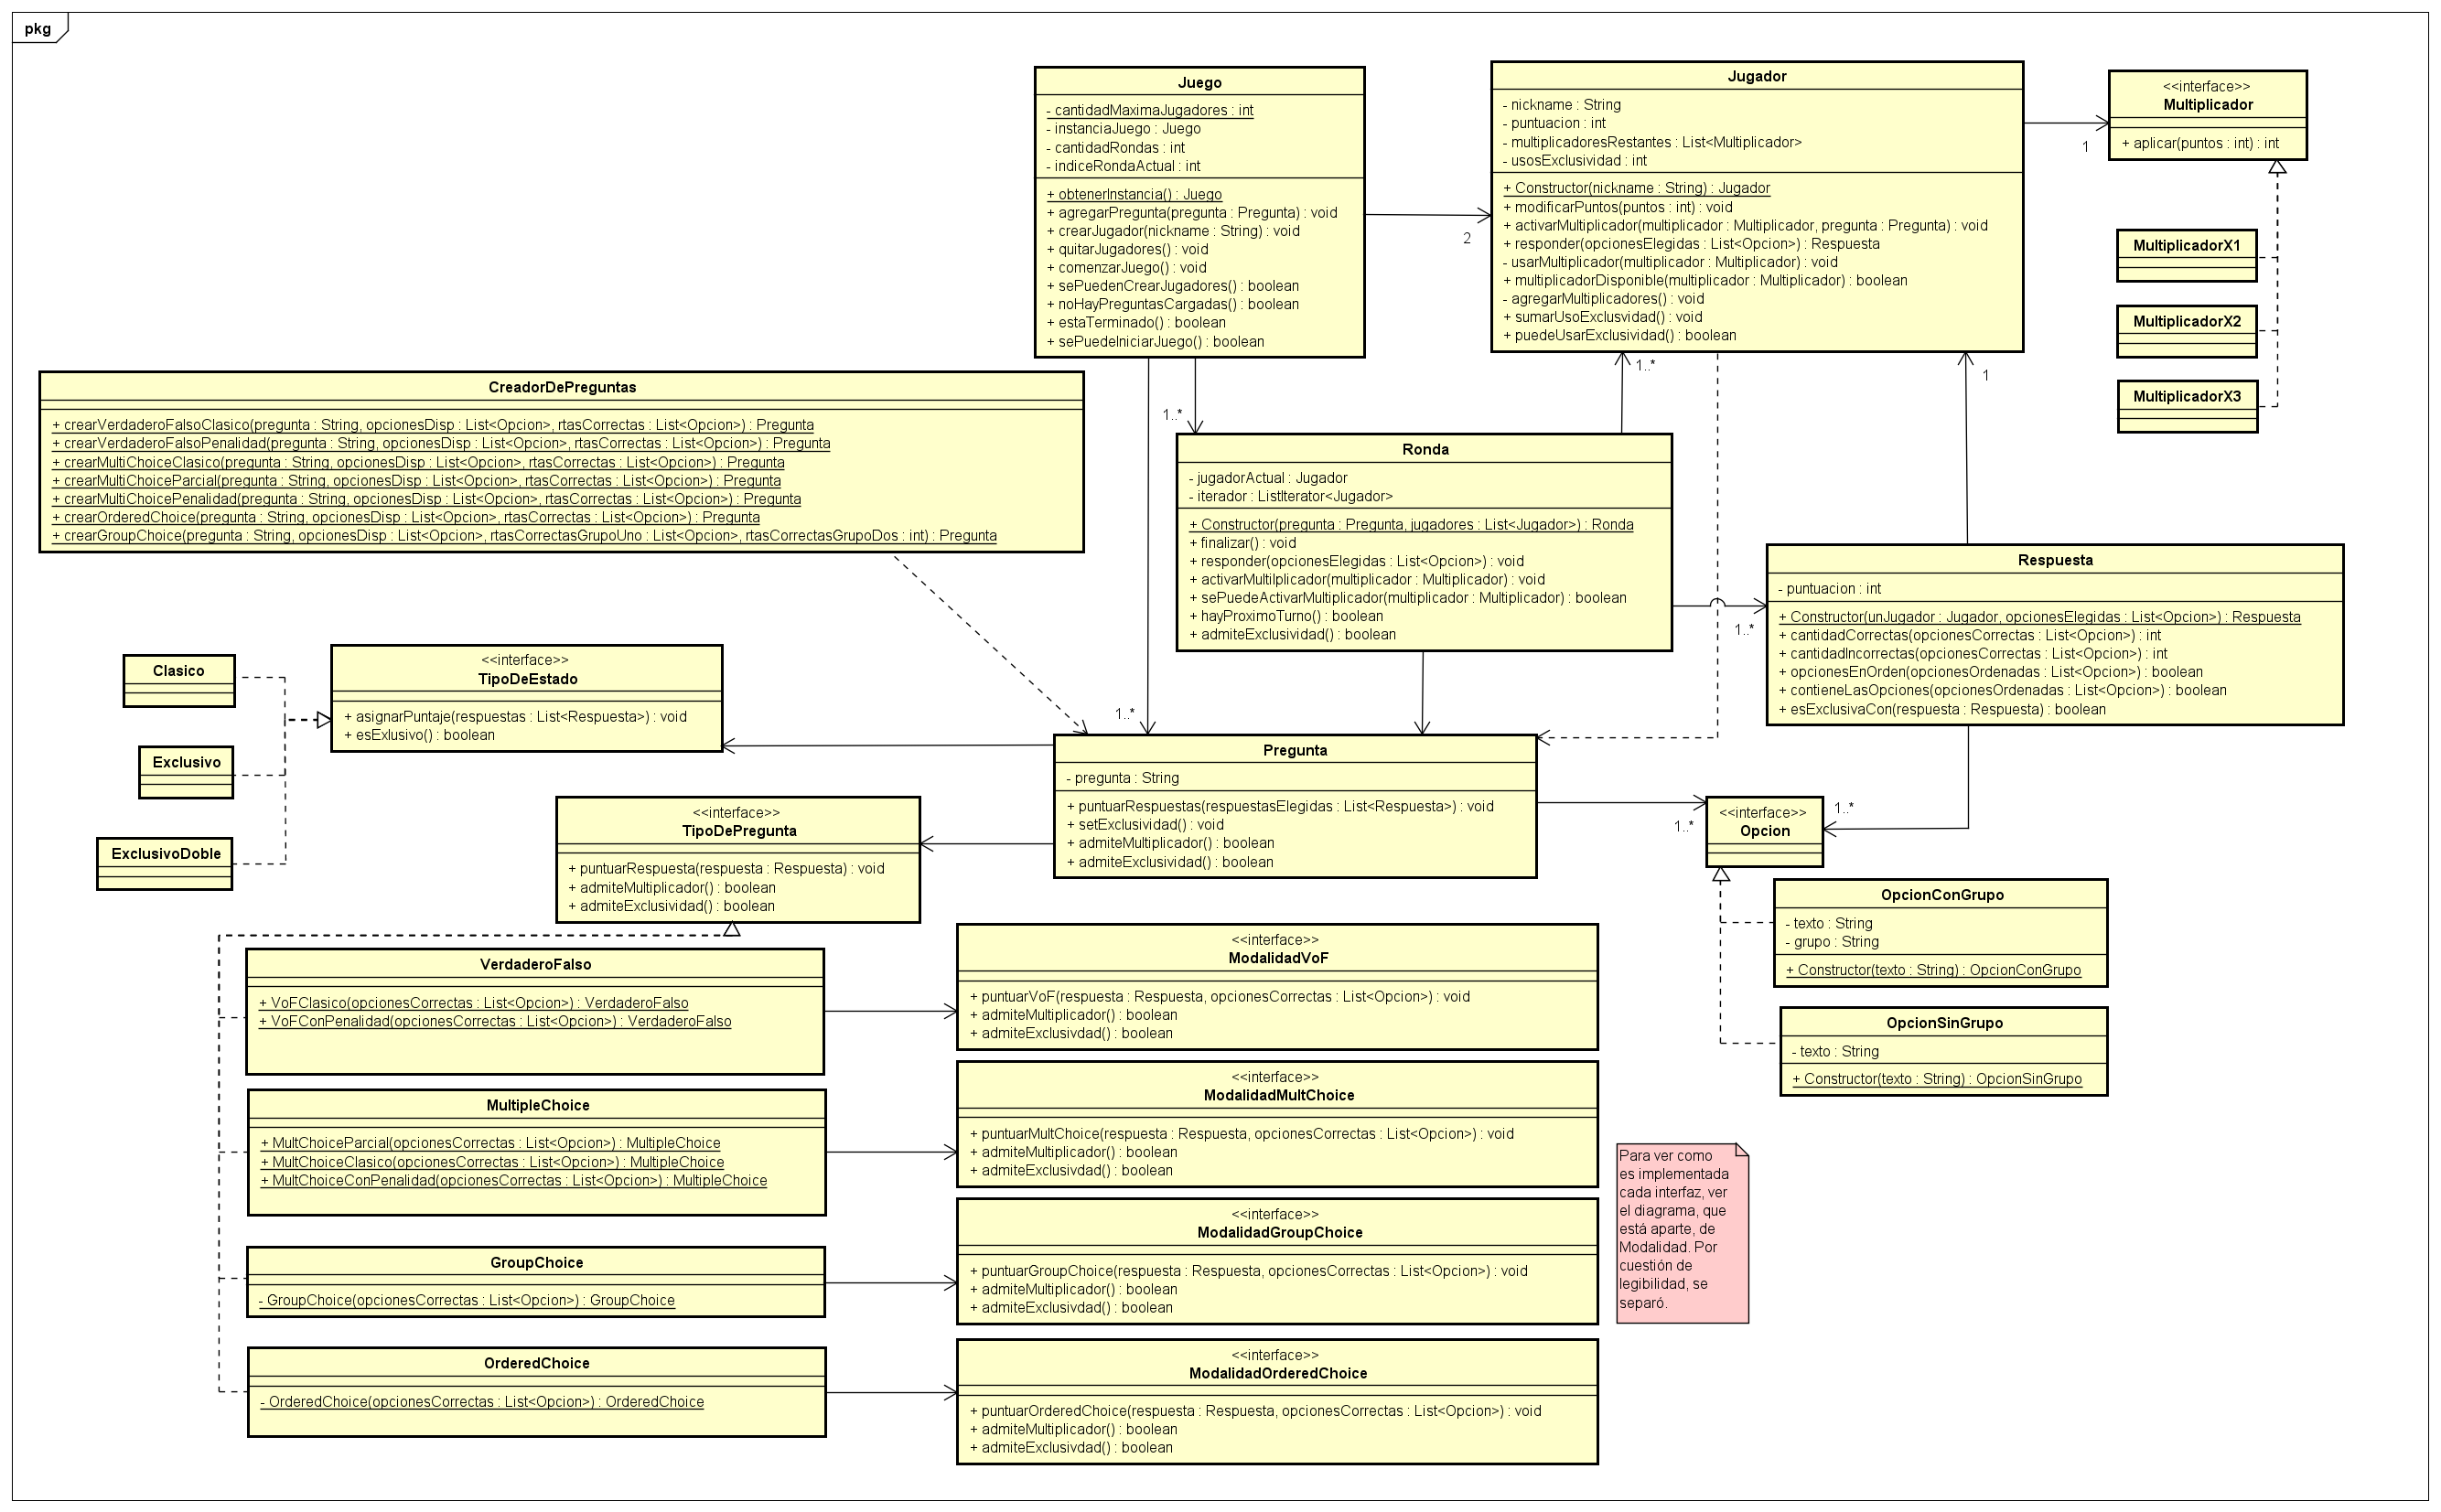
\includegraphics[width=1\textwidth]{img/UMLClases1.png}
\caption{\label{fig:class01}Diagrama de clases general.}
\end{figure}

\newpage
Los siguientes diagramas muestran como las clases núcleo, es decir, las más impórtantes están relacionadas:

\begin{figure}[H]
\centering
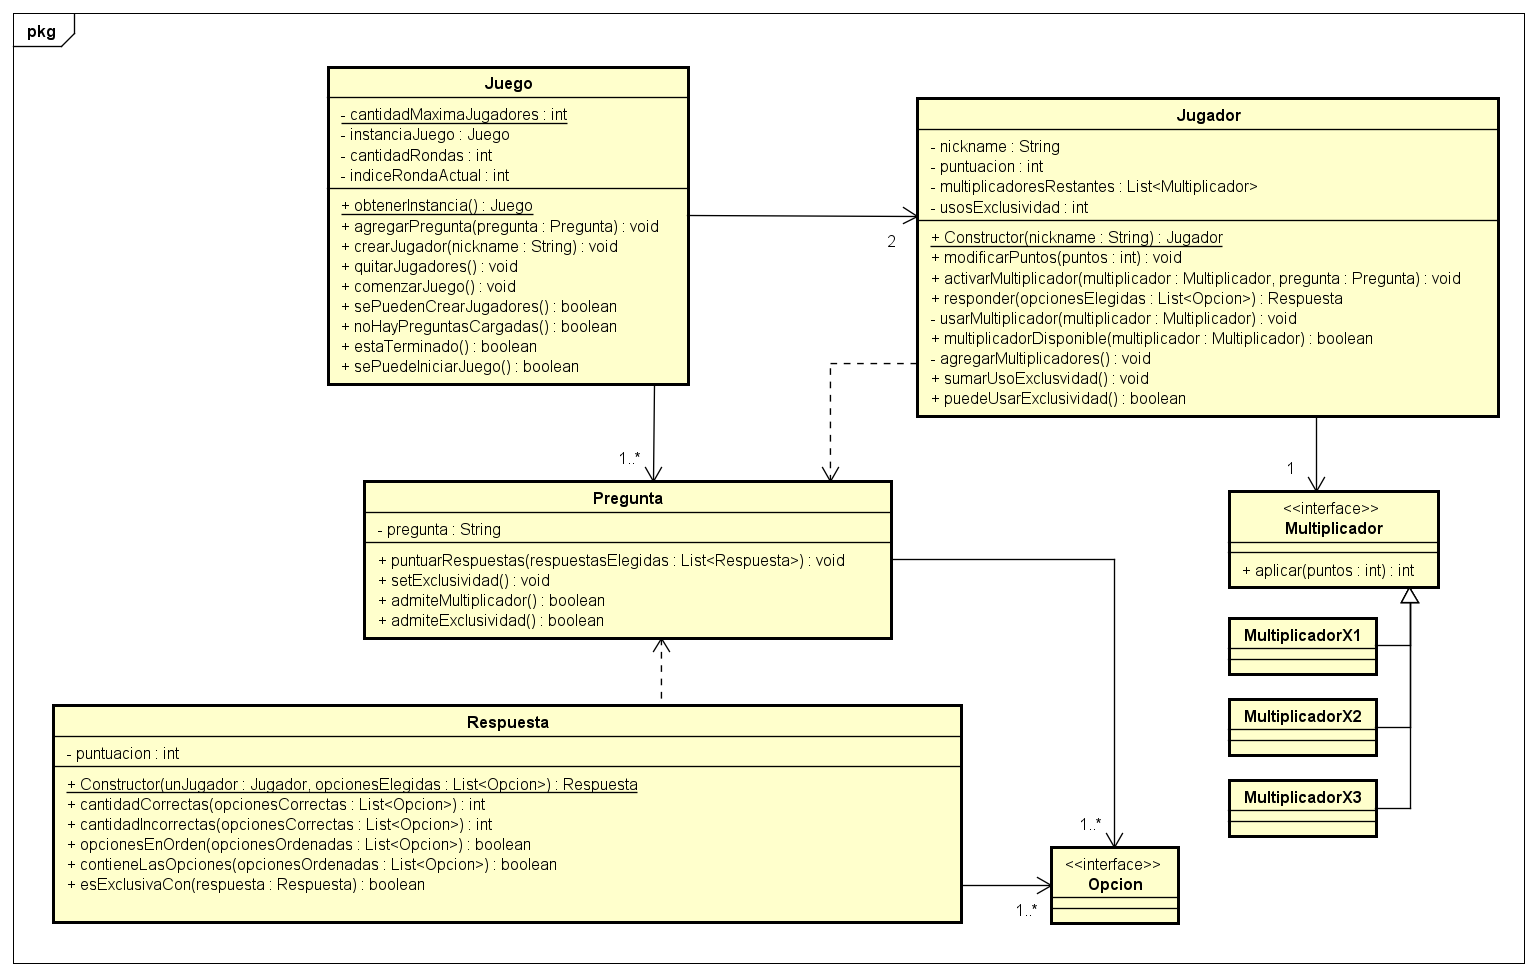
\includegraphics[width=1\textwidth]{img/UMLClases2.png}
\caption{\label{fig:class01}Principales relaciones entre Pregunta, Jugador, Respuesta, Opción, Multiplicador y Juego.}
\end{figure}

\begin{figure}[H]
\centering
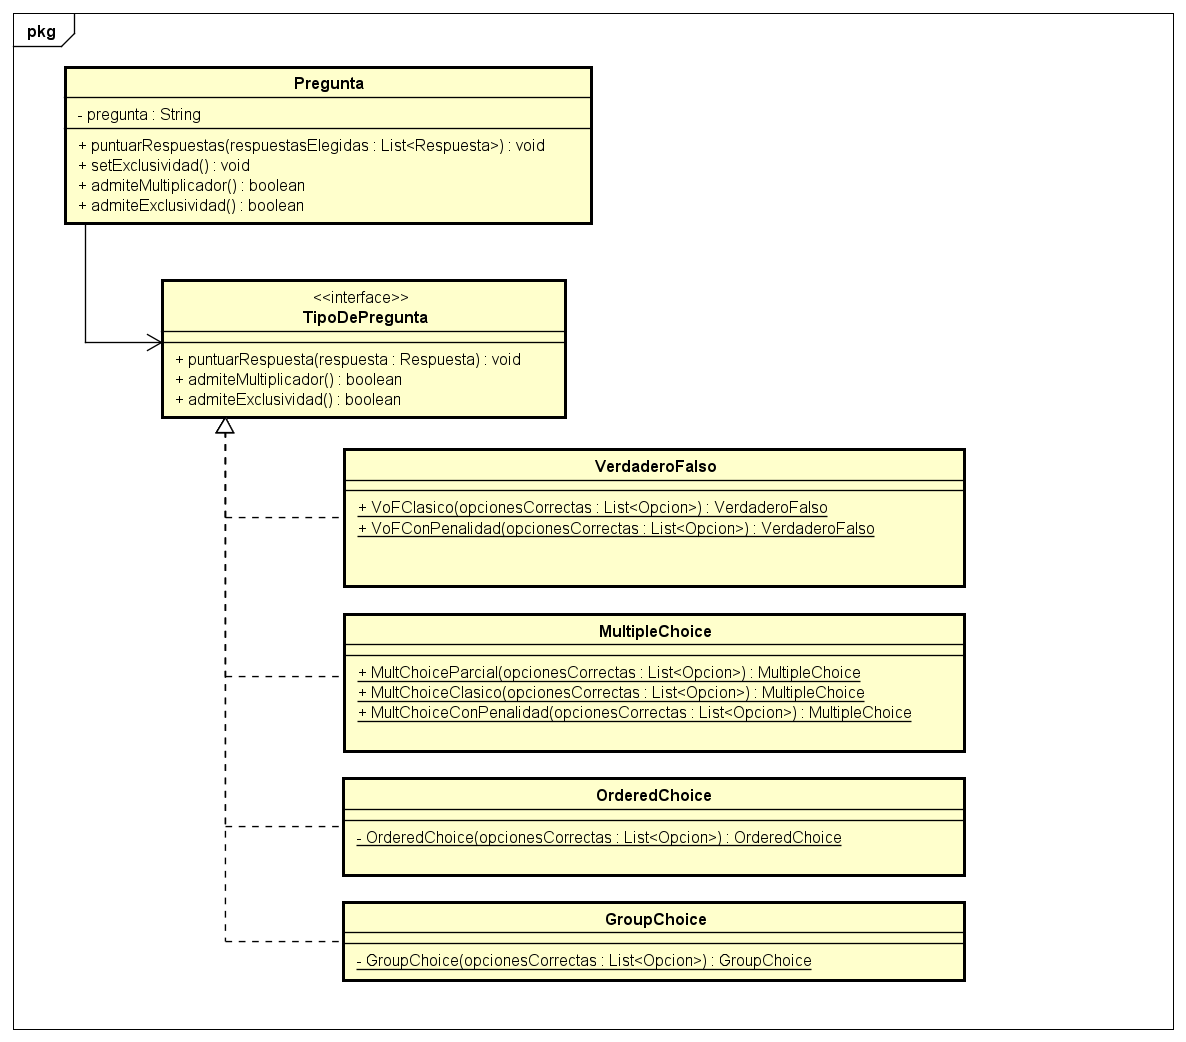
\includegraphics[width=1\textwidth]{img/UMLClases3.png}
\caption{\label{fig:class01}Cada instancia de Pregunta posee un tipoDePregunta, y esta última una instancia de la Modalidad.}
\end{figure}

\newpage
Cada pregunta conoce el tipo de estado actual y este puede ser clásico o exclusivo:

\begin{figure}[H]
\centering
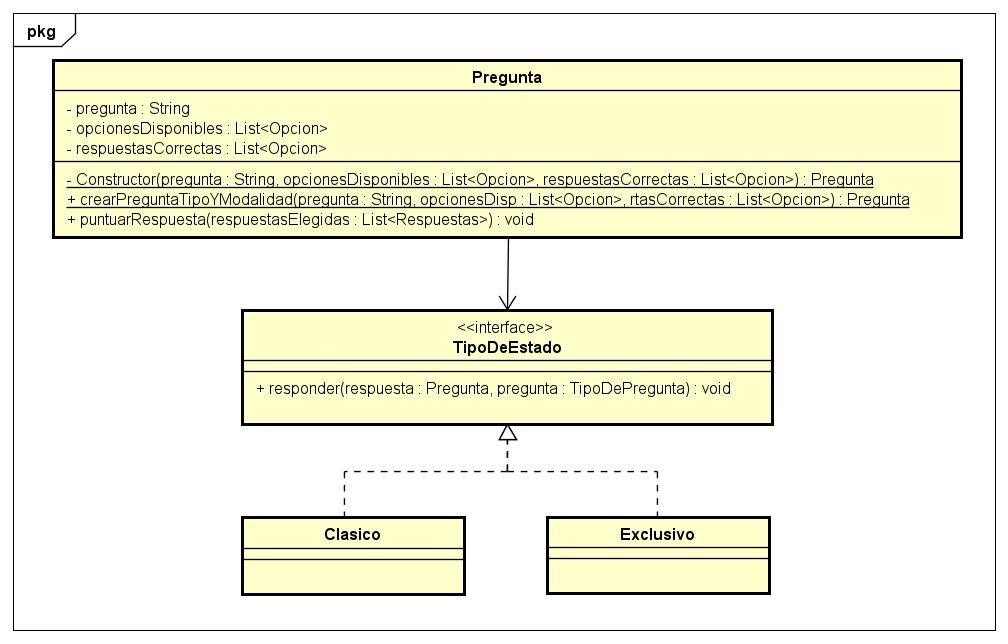
\includegraphics[width=1\textwidth]{img/UMLClases4.png}
\caption{\label{fig:class01}Diagrama de clases.}
\end{figure}

\newpage
\section{Diagramas de Secuencia}

Dejamos a continuación los diagramas de secuencia que muestran las acciones más importantes:

\begin{figure}[H]
\centering
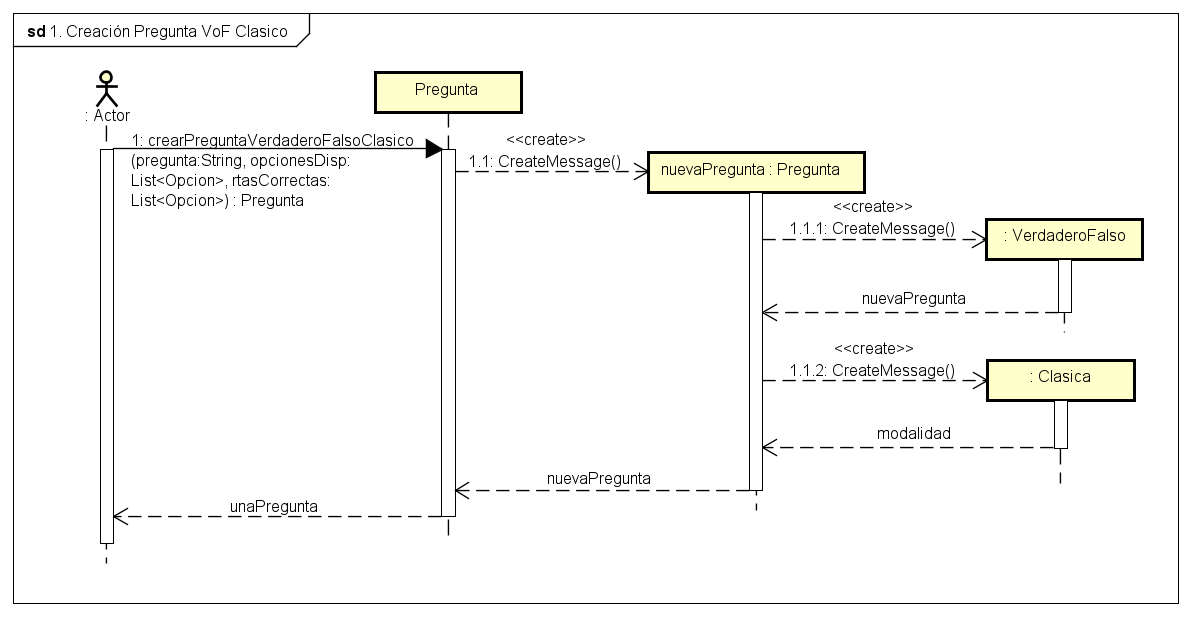
\includegraphics[width=1\textwidth]{img/UMLSeq2.png}
\caption{\label{fig:class01}Creación de la instancia de Pregunta VoF Clasico.}
\end{figure}

\begin{figure}[H]
\centering
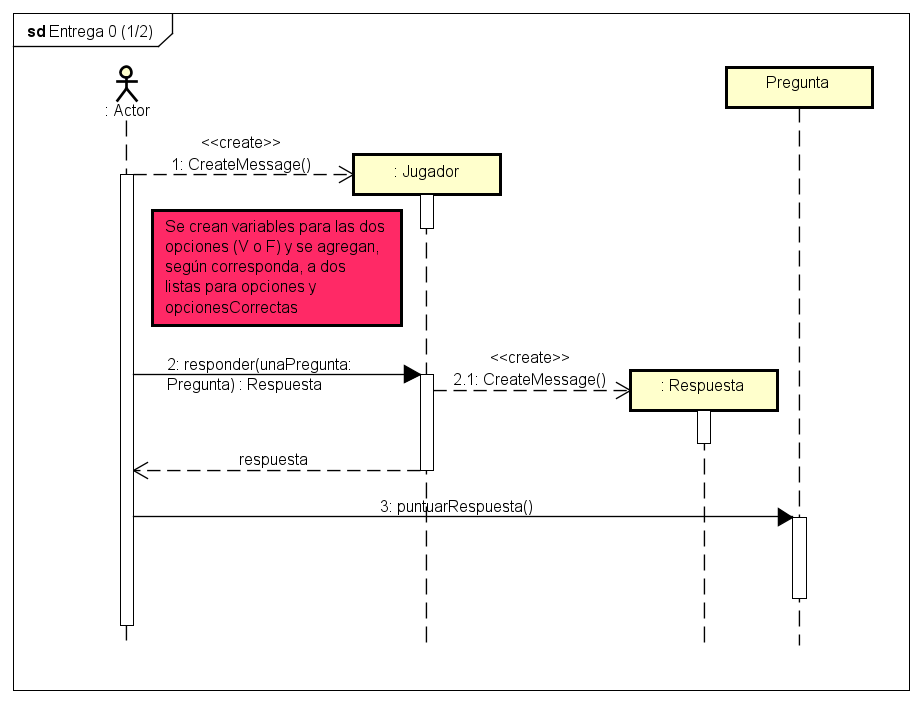
\includegraphics[width=1\textwidth]{img/UMLSeq3.png}
\caption{\label{fig:class01}Evaluado de respuestas de Pregunta VoF Clasico (1/2).}
\end{figure}

\begin{figure}[H]
\centering
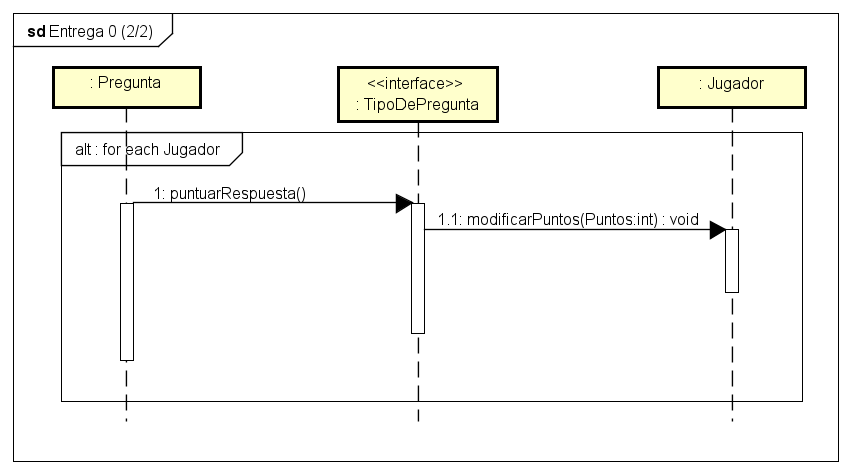
\includegraphics[width=1\textwidth]{img/UMLSeq4.png}
\caption{\label{fig:class01}Evaluado de respuestas de Pregunta VoF Clasico (2/2).}
\end{figure}

\begin{figure}[H]
\centering
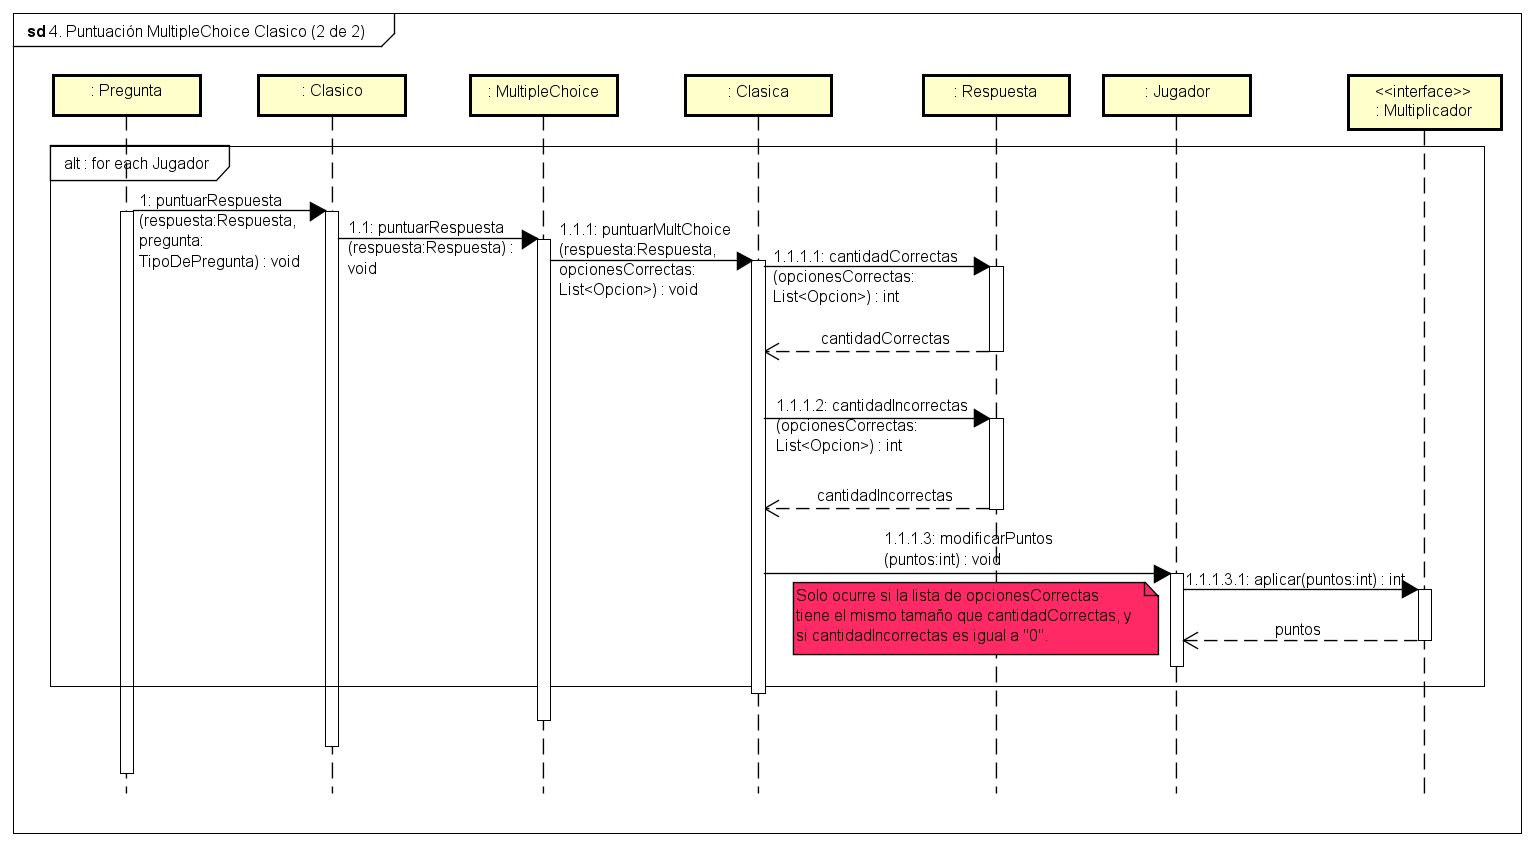
\includegraphics[width=1\textwidth]{img/UMLSeq5.png}
\caption{\label{fig:class01}Evaluado de respuestas de Pregunta Multiple Choice Clasico.}
\end{figure}

\section{Diagrama de Paquetes}
% Explicación concisa del diseño general del trabajo.

No se solicita para esta entrega.

\section{Diagramas de Estados}
% Explicación concisa del diseño general del trabajo.

No se solicita para esta entrega.

\section{Detalles de implementación}
% Explicaciones sobre la implementación interna de algunas clases que consideren que puedan llegar a resultar interesantes.

\subsection{Como se contesta una pregunta}

Una vez que el Jugador selecciona las opciones que desea, se le pide al Jugador que cree una instancia de Respuesta que contenga dichas opciones junto a una referencia al Jugador quien haya instanciado esa respuesta. Luego, esa respuesta es enviada por parametro a la instancia de Pregunta a traves del método puntuarRespuesta.

Luego, la Pregunta hace lo siguiente:

\begin{enumerate}
\item Delega la puntuacion de la respuesta a TipoDePregunta, que a su vez lo delega a la Modalidad(Clasico, Parcial, Penalidad).
\item Modalidad le envia a Respuesta la lista de las opciones correctas y esta devuelve la cantidad de opciones correctas e incorrectas. Modalidad se encarga de darle un puntaje a Respuesta dadas dichas cantidades. El método con el cual Modalidad puntua a la respuesta es exclusivo de cada tipo de Modalidad.
\item Una vez que se tiene la o las respuestas puntuadas, Pregunta se las envía a su Estado(Clasica, Exclusiva o Exclusiva Doble) la cual se encarga de puntuar al Jugador dado los puntajes de las respuestas de los jugadores.
\end{enumerate}

El hecho de que cada objeto Pregunta y TipoDePregunta tenga objetos asociados que definan el comportamiento del mismo (Pregunta tiene Estado y TipoDePregunta, mientras que TipoDePregunta tiene Modalidad), corresponde al patrón de diseño Strategy.

\subsection{Manejo de Turnos}

El modelo cuenta con una clase Ronda, la cual se encarga del manejo de turnos para una pregunta en particular. Cuando se inicia el juego se instancia una Ronda por cada pregunta que se haya añadido al juego. La Ronda se encarga de mandar a puntuar las respuestas, cambiar de turno y de informar si ya no hay jugadores restantes para jugar. Una vez que se indica que no hay jugadores restantes, se mandan a puntuar las respuestas y se cambia de Ronda.

\subsection{Conexión entre el Controlador y el Modelo}

El controlador se encarga de conectar la Vista con el Modelo. Es decir, si se tiene una Vista que muestra los botones que representan las opciones, el controlador se encargara de recolectar las opciones seleccionadas mediante los clicks del usuario con las cuales se crea la instancia de Respuesta del jugador actual y, una vez que hayan respondido todos los jugadores, mandar a puntuar dichas respuestas. Tambien se encarga de modificar la vista teniendo en cuenta las limitaciones del modelo. Por ejemplo, si un jugador no tiene mas multiplicadores disponibles, el controlador se encarga de modificar la vista para que el boton que activa los multiplicadores este desactivado.



\end{document}